\documentclass[a4paper]{article}

\usepackage{arxiv}

\usepackage{fontsize}
\changefontsize{14}

    \usepackage[breakable]{tcolorbox}
    \usepackage{parskip} % Stop auto-indenting (to mimic markdown behaviour)
    

    % Basic figure setup, for now with no caption control since it's done
    % automatically by Pandoc (which extracts ![](path) syntax from Markdown).
    \usepackage{graphicx}
    % Keep aspect ratio if custom image width or height is specified
    \setkeys{Gin}{keepaspectratio}
    % Maintain compatibility with old templates. Remove in nbconvert 6.0
    \let\Oldincludegraphics\includegraphics
    % Ensure that by default, figures have no caption (until we provide a
    % proper Figure object with a Caption API and a way to capture that
    % in the conversion process - todo).
    \usepackage{caption}
    \DeclareCaptionFormat{nocaption}{}
    \captionsetup{format=nocaption,aboveskip=0pt,belowskip=0pt}

    \usepackage{float}
    \floatplacement{figure}{H} % forces figures to be placed at the correct location
    \usepackage{xcolor} % Allow colors to be defined
    \usepackage{enumerate} % Needed for markdown enumerations to work
    \usepackage{geometry} % Used to adjust the document margins
    \usepackage{amsmath} % Equations
    \usepackage{amssymb} % Equations
    \usepackage{textcomp} % defines textquotesingle
    % Hack from http://tex.stackexchange.com/a/47451/13684:
    \AtBeginDocument{%
        \def\PYZsq{\textquotesingle}% Upright quotes in Pygmentized code
    }
    \usepackage{upquote} % Upright quotes for verbatim code
    \usepackage{eurosym} % defines \euro

    \usepackage{iftex}
    \ifPDFTeX
        \usepackage[T1]{fontenc}
        \IfFileExists{alphabeta.sty}{
              \usepackage{alphabeta}
          }{
              \usepackage[mathletters]{ucs}
              \usepackage[utf8x]{inputenc}
          }
    \else
        \usepackage{fontspec}
        \usepackage{unicode-math}
    \fi

    \usepackage{fancyvrb} % verbatim replacement that allows latex
    \usepackage{grffile} % extends the file name processing of package graphics
                         % to support a larger range
    \makeatletter % fix for old versions of grffile with XeLaTeX
    \@ifpackagelater{grffile}{2019/11/01}
    {
      % Do nothing on new versions
    }
    {
      \def\Gread@@xetex#1{%
        \IfFileExists{"\Gin@base".bb}%
        {\Gread@eps{\Gin@base.bb}}%
        {\Gread@@xetex@aux#1}%
      }
    }
    \makeatother
    \usepackage[Export]{adjustbox} % Used to constrain images to a maximum size
    \adjustboxset{max size={0.9\linewidth}{0.9\paperheight}}

    % The hyperref package gives us a pdf with properly built
    % internal navigation ('pdf bookmarks' for the table of contents,
    % internal cross-reference links, web links for URLs, etc.)
    \usepackage{hyperref}
    % The default LaTeX title has an obnoxious amount of whitespace. By default,
    % titling removes some of it. It also provides customization options.
    \usepackage{longtable} % longtable support required by pandoc >1.10
    \usepackage{booktabs}  % table support for pandoc > 1.12.2
    \usepackage{array}     % table support for pandoc >= 2.11.3
    \usepackage{calc}      % table minipage width calculation for pandoc >= 2.11.1
    \usepackage[inline]{enumitem} % IRkernel/repr support (it uses the enumerate* environment)
    \usepackage[normalem]{ulem} % ulem is needed to support strikethroughs (\sout)
                                % normalem makes italics be italics, not underlines
    \usepackage{soul}      % strikethrough (\st) support for pandoc >= 3.0.0
    \usepackage{mathrsfs}
    

    
    % Colors for the hyperref package
    \definecolor{urlcolor}{rgb}{0,.145,.698}
    \definecolor{linkcolor}{rgb}{.71,0.21,0.01}
    \definecolor{citecolor}{rgb}{.12,.54,.11}

    % ANSI colors
    \definecolor{ansi-black}{HTML}{3E424D}
    \definecolor{ansi-black-intense}{HTML}{282C36}
    \definecolor{ansi-red}{HTML}{E75C58}
    \definecolor{ansi-red-intense}{HTML}{B22B31}
    \definecolor{ansi-green}{HTML}{00A250}
    \definecolor{ansi-green-intense}{HTML}{007427}
    \definecolor{ansi-yellow}{HTML}{DDB62B}
    \definecolor{ansi-yellow-intense}{HTML}{B27D12}
    \definecolor{ansi-blue}{HTML}{208FFB}
    \definecolor{ansi-blue-intense}{HTML}{0065CA}
    \definecolor{ansi-magenta}{HTML}{D160C4}
    \definecolor{ansi-magenta-intense}{HTML}{A03196}
    \definecolor{ansi-cyan}{HTML}{60C6C8}
    \definecolor{ansi-cyan-intense}{HTML}{258F8F}
    \definecolor{ansi-white}{HTML}{C5C1B4}
    \definecolor{ansi-white-intense}{HTML}{A1A6B2}
    \definecolor{ansi-default-inverse-fg}{HTML}{FFFFFF}
    \definecolor{ansi-default-inverse-bg}{HTML}{000000}

    % common color for the border for error outputs.
    \definecolor{outerrorbackground}{HTML}{FFDFDF}

    % commands and environments needed by pandoc snippets
    % extracted from the output of `pandoc -s`
    \providecommand{\tightlist}{%
      \setlength{\itemsep}{0pt}\setlength{\parskip}{0pt}}
    \DefineVerbatimEnvironment{Highlighting}{Verbatim}{commandchars=\\\{\}}
    % Add ',fontsize=\small' for more characters per line
    \newenvironment{Shaded}{}{}
    \newcommand{\KeywordTok}[1]{\textcolor[rgb]{0.00,0.44,0.13}{\textbf{{#1}}}}
    \newcommand{\DataTypeTok}[1]{\textcolor[rgb]{0.56,0.13,0.00}{{#1}}}
    \newcommand{\DecValTok}[1]{\textcolor[rgb]{0.25,0.63,0.44}{{#1}}}
    \newcommand{\BaseNTok}[1]{\textcolor[rgb]{0.25,0.63,0.44}{{#1}}}
    \newcommand{\FloatTok}[1]{\textcolor[rgb]{0.25,0.63,0.44}{{#1}}}
    \newcommand{\CharTok}[1]{\textcolor[rgb]{0.25,0.44,0.63}{{#1}}}
    \newcommand{\StringTok}[1]{\textcolor[rgb]{0.25,0.44,0.63}{{#1}}}
    \newcommand{\CommentTok}[1]{\textcolor[rgb]{0.38,0.63,0.69}{\textit{{#1}}}}
    \newcommand{\OtherTok}[1]{\textcolor[rgb]{0.00,0.44,0.13}{{#1}}}
    \newcommand{\AlertTok}[1]{\textcolor[rgb]{1.00,0.00,0.00}{\textbf{{#1}}}}
    \newcommand{\FunctionTok}[1]{\textcolor[rgb]{0.02,0.16,0.49}{{#1}}}
    \newcommand{\RegionMarkerTok}[1]{{#1}}
    \newcommand{\ErrorTok}[1]{\textcolor[rgb]{1.00,0.00,0.00}{\textbf{{#1}}}}
    \newcommand{\NormalTok}[1]{{#1}}

    % Additional commands for more recent versions of Pandoc
    \newcommand{\ConstantTok}[1]{\textcolor[rgb]{0.53,0.00,0.00}{{#1}}}
    \newcommand{\SpecialCharTok}[1]{\textcolor[rgb]{0.25,0.44,0.63}{{#1}}}
    \newcommand{\VerbatimStringTok}[1]{\textcolor[rgb]{0.25,0.44,0.63}{{#1}}}
    \newcommand{\SpecialStringTok}[1]{\textcolor[rgb]{0.73,0.40,0.53}{{#1}}}
    \newcommand{\ImportTok}[1]{{#1}}
    \newcommand{\DocumentationTok}[1]{\textcolor[rgb]{0.73,0.13,0.13}{\textit{{#1}}}}
    \newcommand{\AnnotationTok}[1]{\textcolor[rgb]{0.38,0.63,0.69}{\textbf{\textit{{#1}}}}}
    \newcommand{\CommentVarTok}[1]{\textcolor[rgb]{0.38,0.63,0.69}{\textbf{\textit{{#1}}}}}
    \newcommand{\VariableTok}[1]{\textcolor[rgb]{0.10,0.09,0.49}{{#1}}}
    \newcommand{\ControlFlowTok}[1]{\textcolor[rgb]{0.00,0.44,0.13}{\textbf{{#1}}}}
    \newcommand{\OperatorTok}[1]{\textcolor[rgb]{0.40,0.40,0.40}{{#1}}}
    \newcommand{\BuiltInTok}[1]{{#1}}
    \newcommand{\ExtensionTok}[1]{{#1}}
    \newcommand{\PreprocessorTok}[1]{\textcolor[rgb]{0.74,0.48,0.00}{{#1}}}
    \newcommand{\AttributeTok}[1]{\textcolor[rgb]{0.49,0.56,0.16}{{#1}}}
    \newcommand{\InformationTok}[1]{\textcolor[rgb]{0.38,0.63,0.69}{\textbf{\textit{{#1}}}}}
    \newcommand{\WarningTok}[1]{\textcolor[rgb]{0.38,0.63,0.69}{\textbf{\textit{{#1}}}}}
    \makeatletter
    \newsavebox\pandoc@box
    \newcommand*\pandocbounded[1]{%
      \sbox\pandoc@box{#1}%
      % scaling factors for width and height
      \Gscale@div\@tempa\textheight{\dimexpr\ht\pandoc@box+\dp\pandoc@box\relax}%
      \Gscale@div\@tempb\linewidth{\wd\pandoc@box}%
      % select the smaller of both
      \ifdim\@tempb\p@<\@tempa\p@
        \let\@tempa\@tempb
      \fi
      % scaling accordingly (\@tempa < 1)
      \ifdim\@tempa\p@<\p@
        \scalebox{\@tempa}{\usebox\pandoc@box}%
      % scaling not needed, use as it is
      \else
        \usebox{\pandoc@box}%
      \fi
    }
    \makeatother

    % Define a nice break command that doesn't care if a line doesn't already
    % exist.
    \def\br{\hspace*{\fill} \\* }
    % Math Jax compatibility definitions
    \def\gt{>}
    \def\lt{<}
    \let\Oldtex\TeX
    \let\Oldlatex\LaTeX
    \renewcommand{\TeX}{\textrm{\Oldtex}}
    \renewcommand{\LaTeX}{\textrm{\Oldlatex}}
    
    
    
    
    
    
    
% Pygments definitions
\makeatletter
\def\PY@reset{\let\PY@it=\relax \let\PY@bf=\relax%
    \let\PY@ul=\relax \let\PY@tc=\relax%
    \let\PY@bc=\relax \let\PY@ff=\relax}
\def\PY@tok#1{\csname PY@tok@#1\endcsname}
\def\PY@toks#1+{\ifx\relax#1\empty\else%
    \PY@tok{#1}\expandafter\PY@toks\fi}
\def\PY@do#1{\PY@bc{\PY@tc{\PY@ul{%
    \PY@it{\PY@bf{\PY@ff{#1}}}}}}}
\def\PY#1#2{\PY@reset\PY@toks#1+\relax+\PY@do{#2}}

\@namedef{PY@tok@w}{\def\PY@tc##1{\textcolor[rgb]{0.73,0.73,0.73}{##1}}}
\@namedef{PY@tok@c}{\let\PY@it=\textit\def\PY@tc##1{\textcolor[rgb]{0.24,0.48,0.48}{##1}}}
\@namedef{PY@tok@cp}{\def\PY@tc##1{\textcolor[rgb]{0.61,0.40,0.00}{##1}}}
\@namedef{PY@tok@k}{\let\PY@bf=\textbf\def\PY@tc##1{\textcolor[rgb]{0.00,0.50,0.00}{##1}}}
\@namedef{PY@tok@kp}{\def\PY@tc##1{\textcolor[rgb]{0.00,0.50,0.00}{##1}}}
\@namedef{PY@tok@kt}{\def\PY@tc##1{\textcolor[rgb]{0.69,0.00,0.25}{##1}}}
\@namedef{PY@tok@o}{\def\PY@tc##1{\textcolor[rgb]{0.40,0.40,0.40}{##1}}}
\@namedef{PY@tok@ow}{\let\PY@bf=\textbf\def\PY@tc##1{\textcolor[rgb]{0.67,0.13,1.00}{##1}}}
\@namedef{PY@tok@nb}{\def\PY@tc##1{\textcolor[rgb]{0.00,0.50,0.00}{##1}}}
\@namedef{PY@tok@nf}{\def\PY@tc##1{\textcolor[rgb]{0.00,0.00,1.00}{##1}}}
\@namedef{PY@tok@nc}{\let\PY@bf=\textbf\def\PY@tc##1{\textcolor[rgb]{0.00,0.00,1.00}{##1}}}
\@namedef{PY@tok@nn}{\let\PY@bf=\textbf\def\PY@tc##1{\textcolor[rgb]{0.00,0.00,1.00}{##1}}}
\@namedef{PY@tok@ne}{\let\PY@bf=\textbf\def\PY@tc##1{\textcolor[rgb]{0.80,0.25,0.22}{##1}}}
\@namedef{PY@tok@nv}{\def\PY@tc##1{\textcolor[rgb]{0.10,0.09,0.49}{##1}}}
\@namedef{PY@tok@no}{\def\PY@tc##1{\textcolor[rgb]{0.53,0.00,0.00}{##1}}}
\@namedef{PY@tok@nl}{\def\PY@tc##1{\textcolor[rgb]{0.46,0.46,0.00}{##1}}}
\@namedef{PY@tok@ni}{\let\PY@bf=\textbf\def\PY@tc##1{\textcolor[rgb]{0.44,0.44,0.44}{##1}}}
\@namedef{PY@tok@na}{\def\PY@tc##1{\textcolor[rgb]{0.41,0.47,0.13}{##1}}}
\@namedef{PY@tok@nt}{\let\PY@bf=\textbf\def\PY@tc##1{\textcolor[rgb]{0.00,0.50,0.00}{##1}}}
\@namedef{PY@tok@nd}{\def\PY@tc##1{\textcolor[rgb]{0.67,0.13,1.00}{##1}}}
\@namedef{PY@tok@s}{\def\PY@tc##1{\textcolor[rgb]{0.73,0.13,0.13}{##1}}}
\@namedef{PY@tok@sd}{\let\PY@it=\textit\def\PY@tc##1{\textcolor[rgb]{0.73,0.13,0.13}{##1}}}
\@namedef{PY@tok@si}{\let\PY@bf=\textbf\def\PY@tc##1{\textcolor[rgb]{0.64,0.35,0.47}{##1}}}
\@namedef{PY@tok@se}{\let\PY@bf=\textbf\def\PY@tc##1{\textcolor[rgb]{0.67,0.36,0.12}{##1}}}
\@namedef{PY@tok@sr}{\def\PY@tc##1{\textcolor[rgb]{0.64,0.35,0.47}{##1}}}
\@namedef{PY@tok@ss}{\def\PY@tc##1{\textcolor[rgb]{0.10,0.09,0.49}{##1}}}
\@namedef{PY@tok@sx}{\def\PY@tc##1{\textcolor[rgb]{0.00,0.50,0.00}{##1}}}
\@namedef{PY@tok@m}{\def\PY@tc##1{\textcolor[rgb]{0.40,0.40,0.40}{##1}}}
\@namedef{PY@tok@gh}{\let\PY@bf=\textbf\def\PY@tc##1{\textcolor[rgb]{0.00,0.00,0.50}{##1}}}
\@namedef{PY@tok@gu}{\let\PY@bf=\textbf\def\PY@tc##1{\textcolor[rgb]{0.50,0.00,0.50}{##1}}}
\@namedef{PY@tok@gd}{\def\PY@tc##1{\textcolor[rgb]{0.63,0.00,0.00}{##1}}}
\@namedef{PY@tok@gi}{\def\PY@tc##1{\textcolor[rgb]{0.00,0.52,0.00}{##1}}}
\@namedef{PY@tok@gr}{\def\PY@tc##1{\textcolor[rgb]{0.89,0.00,0.00}{##1}}}
\@namedef{PY@tok@ge}{\let\PY@it=\textit}
\@namedef{PY@tok@gs}{\let\PY@bf=\textbf}
\@namedef{PY@tok@ges}{\let\PY@bf=\textbf\let\PY@it=\textit}
\@namedef{PY@tok@gp}{\let\PY@bf=\textbf\def\PY@tc##1{\textcolor[rgb]{0.00,0.00,0.50}{##1}}}
\@namedef{PY@tok@go}{\def\PY@tc##1{\textcolor[rgb]{0.44,0.44,0.44}{##1}}}
\@namedef{PY@tok@gt}{\def\PY@tc##1{\textcolor[rgb]{0.00,0.27,0.87}{##1}}}
\@namedef{PY@tok@err}{\def\PY@bc##1{{\setlength{\fboxsep}{\string -\fboxrule}\fcolorbox[rgb]{1.00,0.00,0.00}{1,1,1}{\strut ##1}}}}
\@namedef{PY@tok@kc}{\let\PY@bf=\textbf\def\PY@tc##1{\textcolor[rgb]{0.00,0.50,0.00}{##1}}}
\@namedef{PY@tok@kd}{\let\PY@bf=\textbf\def\PY@tc##1{\textcolor[rgb]{0.00,0.50,0.00}{##1}}}
\@namedef{PY@tok@kn}{\let\PY@bf=\textbf\def\PY@tc##1{\textcolor[rgb]{0.00,0.50,0.00}{##1}}}
\@namedef{PY@tok@kr}{\let\PY@bf=\textbf\def\PY@tc##1{\textcolor[rgb]{0.00,0.50,0.00}{##1}}}
\@namedef{PY@tok@bp}{\def\PY@tc##1{\textcolor[rgb]{0.00,0.50,0.00}{##1}}}
\@namedef{PY@tok@fm}{\def\PY@tc##1{\textcolor[rgb]{0.00,0.00,1.00}{##1}}}
\@namedef{PY@tok@vc}{\def\PY@tc##1{\textcolor[rgb]{0.10,0.09,0.49}{##1}}}
\@namedef{PY@tok@vg}{\def\PY@tc##1{\textcolor[rgb]{0.10,0.09,0.49}{##1}}}
\@namedef{PY@tok@vi}{\def\PY@tc##1{\textcolor[rgb]{0.10,0.09,0.49}{##1}}}
\@namedef{PY@tok@vm}{\def\PY@tc##1{\textcolor[rgb]{0.10,0.09,0.49}{##1}}}
\@namedef{PY@tok@sa}{\def\PY@tc##1{\textcolor[rgb]{0.73,0.13,0.13}{##1}}}
\@namedef{PY@tok@sb}{\def\PY@tc##1{\textcolor[rgb]{0.73,0.13,0.13}{##1}}}
\@namedef{PY@tok@sc}{\def\PY@tc##1{\textcolor[rgb]{0.73,0.13,0.13}{##1}}}
\@namedef{PY@tok@dl}{\def\PY@tc##1{\textcolor[rgb]{0.73,0.13,0.13}{##1}}}
\@namedef{PY@tok@s2}{\def\PY@tc##1{\textcolor[rgb]{0.73,0.13,0.13}{##1}}}
\@namedef{PY@tok@sh}{\def\PY@tc##1{\textcolor[rgb]{0.73,0.13,0.13}{##1}}}
\@namedef{PY@tok@s1}{\def\PY@tc##1{\textcolor[rgb]{0.73,0.13,0.13}{##1}}}
\@namedef{PY@tok@mb}{\def\PY@tc##1{\textcolor[rgb]{0.40,0.40,0.40}{##1}}}
\@namedef{PY@tok@mf}{\def\PY@tc##1{\textcolor[rgb]{0.40,0.40,0.40}{##1}}}
\@namedef{PY@tok@mh}{\def\PY@tc##1{\textcolor[rgb]{0.40,0.40,0.40}{##1}}}
\@namedef{PY@tok@mi}{\def\PY@tc##1{\textcolor[rgb]{0.40,0.40,0.40}{##1}}}
\@namedef{PY@tok@il}{\def\PY@tc##1{\textcolor[rgb]{0.40,0.40,0.40}{##1}}}
\@namedef{PY@tok@mo}{\def\PY@tc##1{\textcolor[rgb]{0.40,0.40,0.40}{##1}}}
\@namedef{PY@tok@ch}{\let\PY@it=\textit\def\PY@tc##1{\textcolor[rgb]{0.24,0.48,0.48}{##1}}}
\@namedef{PY@tok@cm}{\let\PY@it=\textit\def\PY@tc##1{\textcolor[rgb]{0.24,0.48,0.48}{##1}}}
\@namedef{PY@tok@cpf}{\let\PY@it=\textit\def\PY@tc##1{\textcolor[rgb]{0.24,0.48,0.48}{##1}}}
\@namedef{PY@tok@c1}{\let\PY@it=\textit\def\PY@tc##1{\textcolor[rgb]{0.24,0.48,0.48}{##1}}}
\@namedef{PY@tok@cs}{\let\PY@it=\textit\def\PY@tc##1{\textcolor[rgb]{0.24,0.48,0.48}{##1}}}

\def\PYZbs{\char`\\}
\def\PYZus{\char`\_}
\def\PYZob{\char`\{}
\def\PYZcb{\char`\}}
\def\PYZca{\char`\^}
\def\PYZam{\char`\&}
\def\PYZlt{\char`\<}
\def\PYZgt{\char`\>}
\def\PYZsh{\char`\#}
\def\PYZpc{\char`\%}
\def\PYZdl{\char`\$}
\def\PYZhy{\char`\-}
\def\PYZsq{\char`\'}
\def\PYZdq{\char`\"}
\def\PYZti{\char`\~}
% for compatibility with earlier versions
\def\PYZat{@}
\def\PYZlb{[}
\def\PYZrb{]}
\makeatother


    % For linebreaks inside Verbatim environment from package fancyvrb.
    \makeatletter
        \newbox\Wrappedcontinuationbox
        \newbox\Wrappedvisiblespacebox
        \newcommand*\Wrappedvisiblespace {\textcolor{red}{\textvisiblespace}}
        \newcommand*\Wrappedcontinuationsymbol {\textcolor{red}{\llap{\tiny$\m@th\hookrightarrow$}}}
        \newcommand*\Wrappedcontinuationindent {3ex }
        \newcommand*\Wrappedafterbreak {\kern\Wrappedcontinuationindent\copy\Wrappedcontinuationbox}
        % Take advantage of the already applied Pygments mark-up to insert
        % potential linebreaks for TeX processing.
        %        {, <, #, %, $, ' and ": go to next line.
        %        _, }, ^, &, >, - and ~: stay at end of broken line.
        % Use of \textquotesingle for straight quote.
        \newcommand*\Wrappedbreaksatspecials {%
            \def\PYGZus{\discretionary{\char`\_}{\Wrappedafterbreak}{\char`\_}}%
            \def\PYGZob{\discretionary{}{\Wrappedafterbreak\char`\{}{\char`\{}}%
            \def\PYGZcb{\discretionary{\char`\}}{\Wrappedafterbreak}{\char`\}}}%
            \def\PYGZca{\discretionary{\char`\^}{\Wrappedafterbreak}{\char`\^}}%
            \def\PYGZam{\discretionary{\char`\&}{\Wrappedafterbreak}{\char`\&}}%
            \def\PYGZlt{\discretionary{}{\Wrappedafterbreak\char`\<}{\char`\<}}%
            \def\PYGZgt{\discretionary{\char`\>}{\Wrappedafterbreak}{\char`\>}}%
            \def\PYGZsh{\discretionary{}{\Wrappedafterbreak\char`\#}{\char`\#}}%
            \def\PYGZpc{\discretionary{}{\Wrappedafterbreak\char`\%}{\char`\%}}%
            \def\PYGZdl{\discretionary{}{\Wrappedafterbreak\char`\$}{\char`\$}}%
            \def\PYGZhy{\discretionary{\char`\-}{\Wrappedafterbreak}{\char`\-}}%
            \def\PYGZsq{\discretionary{}{\Wrappedafterbreak\textquotesingle}{\textquotesingle}}%
            \def\PYGZdq{\discretionary{}{\Wrappedafterbreak\char`\"}{\char`\"}}%
            \def\PYGZti{\discretionary{\char`\~}{\Wrappedafterbreak}{\char`\~}}%
        }
        % Some characters . , ; ? ! / are not pygmentized.
        % This macro makes them "active" and they will insert potential linebreaks
        \newcommand*\Wrappedbreaksatpunct {%
            \lccode`\~`\.\lowercase{\def~}{\discretionary{\hbox{\char`\.}}{\Wrappedafterbreak}{\hbox{\char`\.}}}%
            \lccode`\~`\,\lowercase{\def~}{\discretionary{\hbox{\char`\,}}{\Wrappedafterbreak}{\hbox{\char`\,}}}%
            \lccode`\~`\;\lowercase{\def~}{\discretionary{\hbox{\char`\;}}{\Wrappedafterbreak}{\hbox{\char`\;}}}%
            \lccode`\~`\:\lowercase{\def~}{\discretionary{\hbox{\char`\:}}{\Wrappedafterbreak}{\hbox{\char`\:}}}%
            \lccode`\~`\?\lowercase{\def~}{\discretionary{\hbox{\char`\?}}{\Wrappedafterbreak}{\hbox{\char`\?}}}%
            \lccode`\~`\!\lowercase{\def~}{\discretionary{\hbox{\char`\!}}{\Wrappedafterbreak}{\hbox{\char`\!}}}%
            \lccode`\~`\/\lowercase{\def~}{\discretionary{\hbox{\char`\/}}{\Wrappedafterbreak}{\hbox{\char`\/}}}%
            \catcode`\.\active
            \catcode`\,\active
            \catcode`\;\active
            \catcode`\:\active
            \catcode`\?\active
            \catcode`\!\active
            \catcode`\/\active
            \lccode`\~`\~
        }
    \makeatother

    \let\OriginalVerbatim=\Verbatim
    \makeatletter
    \renewcommand{\Verbatim}[1][1]{%
        %\parskip\z@skip
        \sbox\Wrappedcontinuationbox {\Wrappedcontinuationsymbol}%
        \sbox\Wrappedvisiblespacebox {\FV@SetupFont\Wrappedvisiblespace}%
        \def\FancyVerbFormatLine ##1{\hsize\linewidth
            \vtop{\raggedright\hyphenpenalty\z@\exhyphenpenalty\z@
                \doublehyphendemerits\z@\finalhyphendemerits\z@
                \strut ##1\strut}%
        }%
        % If the linebreak is at a space, the latter will be displayed as visible
        % space at end of first line, and a continuation symbol starts next line.
        % Stretch/shrink are however usually zero for typewriter font.
        \def\FV@Space {%
            \nobreak\hskip\z@ plus\fontdimen3\font minus\fontdimen4\font
            \discretionary{\copy\Wrappedvisiblespacebox}{\Wrappedafterbreak}
            {\kern\fontdimen2\font}%
        }%

        % Allow breaks at special characters using \PYG... macros.
        \Wrappedbreaksatspecials
        % Breaks at punctuation characters . , ; ? ! and / need catcode=\active
        \OriginalVerbatim[#1,codes*=\Wrappedbreaksatpunct]%
    }
    \makeatother

    % Exact colors from NB
    \definecolor{incolor}{HTML}{303F9F}
    \definecolor{outcolor}{HTML}{D84315}
    \definecolor{cellborder}{HTML}{CFCFCF}
    \definecolor{cellbackground}{HTML}{F7F7F7}

    % prompt
    \makeatletter
    \newcommand{\boxspacing}{\kern\kvtcb@left@rule\kern\kvtcb@boxsep}
    \makeatother
    \newcommand{\prompt}[4]{
        {\ttfamily\llap{{\color{#2}[#3]:\hspace{3pt}#4}}\vspace{-\baselineskip}}
    }
    

    
    % Prevent overflowing lines due to hard-to-break entities
    \sloppy
    % Setup hyperref package
    \hypersetup{
      breaklinks=true,  % so long urls are correctly broken across lines
      colorlinks=true,
      urlcolor=urlcolor,
      linkcolor=linkcolor,
      citecolor=citecolor,
      }
    % Slightly bigger margins than the latex defaults
    
    \geometry{verbose,tmargin=1in,bmargin=1in,lmargin=1in,rmargin=1in}


    
  
\title{Analyse Détaillée de Mixture-of-Recursions (MoE)}


\author{
 Mokira \\
  % School of Coumputing and Information\\
  % University of Pittsburgh\\
  % Pittsburgh, PA 15213 \\
  % \texttt{dr.mokira@gmail.com} \\
  Ingénieur Machine Learning \\
  (+229) 019 798 5109 \\
  \texttt{dr.mokira@gmail.com} \\
  %% \AND
  %% Coauthor \\
  %% Affiliation \\
  %% Address \\
  %% \texttt{email} \\
  %% \And
  %% Coauthor \\
  %% Affiliation \\
  %% Address \\
  %% \texttt{email} \\
  %% \And
  %% Coauthor \\
  %% Affiliation \\
  %% Address \\
  %% \texttt{email} \\
}

\begin{document}
\maketitle

\begin{abstract}
% Pourquoi MoR est une petite révolution ?
% Imaginez un modèle de langage qui combine l’efficacité mémoire
% des architectures à partage de paramètres (comme ALBERT) avec l’intelligence
% computationnelle du calcul adaptatif (comme Mixture-of-Depths) :
% c’est exactement ce que propose Mixture-of-Recursions (MoR).
% Au lieu d’utiliser des couches distinctes, MoR réutilise un même bloc
% de calcul de manière récursive, tandis qu’un routeur léger décide
% dynamiquement pour chaque mot s’il doit « sortir » rapidement ou "réfléchir"
% plus longtemps en passant par des recursions supplémentaires. Résultat ?
% Une réduction simultanée de la taille du modèle (-50\% de paramètres),
% du temps de calcul (meilleur débit d’inférence) et de la mémoire cache,
% sans sacrifier la performance --- ouvrant la voie à des LLMs à la fois agiles,
% économiques et puissants. Une avancée architecturale majeure qui mérite
% d’être explorée dans les moindres détails !

%  Dans cette recherche, on cherche à garder
% la performance des gros modèles, mais sans payer des prix énormes. Il existe
% des techniques pour rendre les modèles plus efficaces : \textbf{Parameter
% sharing} pour réduire la taille du modèle et \textbf{Adaptive computation}
% pour réduire le temps d’inférence (temps de calcule). Mais jusqu’à maintenant,
% les chercheurs faisaient soit l’un, soit l’autre, pas les deux en même temps.
% Ce qui est un problème. C'est qu'on introduit une nouvelle technique appellée
% \textbf{MoR (Mixture-of-Recursions)}. Il s'agit d'une approache qui mélange
% le partage de paramètres (recursive transformer) et le calcul adaptatif
% (adaptive computation). L’idée est donc de prendre le meilleur
% des deux mondes. MoR utilise les mêmes couches plusieurs fois en faisant
% de la récursivité. Un petit module appelé \textit{router} décide,
% pour chaque token, combien de fois il doit passer par la pile de couches,
% de tel sorte que les tokens faciles se retrouvent avec peu de recursion
% et les tokens difficiles se retrouvent avec plus de recursion.
% L'opération du mécanisme d'attention est très coûteuse car elle nécessite
% que chaque token regarde tous les autres (complexité quadratique).
% Or, grâce à la MoR, à chaque récursion, seuls les tokens encore actifs
% (pas sortis) continuent à calculer leur score attention.
% Les autres (déjà sortis) ne participent plus, ce qui nous permet d'économiser
% du temps. En plus, MoR ne stocke en mémoire que les clés/valeurs (KV cache)
% des tokens actifs. La MoR indroduit \textbf{KV sharing}
% qui nous permet d'éviter de recalculer et de stocker des KV (key-values)
% pour chaque récursion, du coup, on réutilise ceux calculés dès
% la première fois. Ce qui reduit les coûts de calcule au moment où on encode
% tout le contexte (\textit{prefill}) avant de générer et réduit l'espace
% en mémoire.

Quand on augmente la taille des modèles de langage (plus de couches,
plus de paramètres, plus de données), ils deviennent plus performant
et intelligents. Mais en contrepartie, leur entraînement coûte énormément
(des semaines de GPU), et leur utilisation (en inférence) demande beaucoup 
de mémoire et de puissance de calcul.
Mixture-of-Recursions (MoR) propose une nouvelle façon de rendre les modèles
de langue à la fois plus performant et moins coûteux.
Au lieu d’augmenter indéfiniment la taille des modèles — ce qui entraîne
des besoins énormes en calcul et en mémoire — MoR combine deux approches
qui ont toujours été séparées jusqu'ici. Il s'agit du partage de paramètres
et du calcul adaptatif par jeton.
Concrètement, le modèle réutilise un même bloc de couches plusieurs fois
(comme une pile de récursions) pour économiser des paramètres,
et utilise un module léger appelé routeur qui décident dynamiquement
combien d’étapes de calcul chaque jeton doit parcourir.
ce qui réduit le coût mémoire et accélère les calculs grâce
à un cache sélectif des clés-valeurs. Une variante introduit aussi le partage 
des clés-valeurs du premier passage (\textit{KV sharing}), réduisant fortement
la latence et l’empreint mémoire lors du préremplissage.
Résultat : avec moins de paramètres et moins de coûts de calcul,
MoR atteint une meilleure perplexité et de meilleures performances
few-shot que les Transformers classiques.
\end{abstract}


% keywords can be removed
%\keywords{First keyword \and Second keyword \and More}

\newpage
\tableofcontents
\newpage

\section{Introduction}
Aujourd'hui, les intelligences artificielles qui comprennent et génèrent
du langage, comme celles qui animent les assistants virtuels, reposent
sur des architectures dites « Transformers ». Si elles sont impressionnantes,
leur formidable puissance a un coût : une gourmandise excessive en calcul
et en mémoire. Pour fonctionner, ces modèles doivent en effet traiter
chaque mot d'un texte avec la même intensité. Par exemple, pour comprendre
un mot complexe comme « philosophique », un modèle de langue doit lui accorder
autant de temps et de ressources qu’à un mot simple comme « le » ou « et ».
Cette approche uniforme est coûteuse et inefficace.

Les LLMs sont puissants, mais gourmands en mémoire et en calcul.
Et si on pouvait créer un modèle à la fois compact et intelligent,
capable de concentrer ses efforts sur les mots qui en valent vraiment
la peine ?

C'est la réponse à cette question qui a donné naissance
à la \textbf{Mixture-of-Recursions (MoR)}. une nouvelle architecture
qui permet à un modèle de langage d'allouer intelligemment son « effort
de calcul » de manière adaptive, token par token. Imaginez une usine
de traitement où les produits simples sont expédiés rapidement
après une étape, tandis que les produits complexes passent
par plusieurs stations de contrôle pour un travail approfondi.
MoR opère de la même façon : en réutilisant un même groupe de couches
de neurones de manière recursive, et en utilisant un mécanisme de décision
légère pour déterminer quels mots méritent plus de « réflexion ».
Cette méthode unifie pour la première fois les gains en efficacité
mémoire (moins de paramètres) et en efficacité computationnelle
(moins de calculs superflus), sans compromettre les performances.

Dans ce didacticiel, nous commencerons par un rappel des concepts
fondamentaux nécessaires à la compréhension. Ensuite, nous définirons
précisément le problème qui se pose. Puis, nous détaillerons
le fonctionnement de la solution proposée par MoR pour résoudre le problème,
Nous illustrerons cette solution par des exemples concrets
et une implémentation simplifiée en Python.
Nous discuterons ensuite des apports majeurs et des limites de cette solution,
et proposerons des pistes d'amélioration futures,
et enfin conclure sur la portée de ce travail.

\section{Connaissances de Base Nécessaires}
\label{sec:base}
Pour comprendre ce papier, il faut se familiariser avec quelques concepts
clés des modèles de type Transformers.

\subsection{Architecture Transformer de base (Vaswani et al., 2017)}
Un transformer est un modèle de réseau de neurones qui utilise
des \textbf{mécanismes d'attention} pour traiter des séquences de données
(comme du texte). Il est composé de couches (layers)
empilées les unes sur les autres. Chaque couche a une \textbf{auto-attention}
et un réseau \textbf{feed-forward}.

Imaginez un Transformer comme une usine avec plusieurs étages (couches/layers).
Chaque étage traite l'information et la passe à l'étage suivant.
Dans un modèle traditionnel comme GPT :

Entrée : "Le chat mange" $\rightarrow$ Couche $1$ $\rightarrow$ Couche $2$
$\rightarrow \ldots \rightarrow $  Couche $N$ → Sortie : "le poisson"

À chaque étage, chaque mot (token) regarde tous les autres mots pour mieux
se comprendre soi-même (c'est l'auto-attention), puis une petite usine interne
(le feed-forward) pour calculer sa représentation.

\subsection{Cache KV (Key-Value Cache)}
Pour générer du texte de manière autoregressive (un mot à la fois),
on doit éviter de recalculer les représentations des mots passés
à chaque nouvelle étape. Le cache KV stocke les "clés" et "valeurs" de tous
les mots déjà générés, ce qui rend le processus beaucoup plus rapide.

De façon analogique, lorsque vous lisez un livre, vous n'oubliez
pas les chapitres précédents. Votre cerveau garde en cache les informations
importantes. Le cache KV fait la même chose pour le modèle.

\subsection{Partage de Paramètres (Parameter Sharing)}
Au lieu d'avoir des poids uniques pour chaque couche, on utilise le même jeu
de poids pour plusieurs couches. Cela réduit énormément la taille du modèle.

Exemple : Au lieu d'avoir 24 stations de travail différentes dans notre usine,
on n'en a que 8, mais on fait passer la phrase 3 fois par les mêmes 8 stations.
L'usine est plus petite (moins de paramètres) mais le travail est tout aussi
profond (3 passages = 24 traitements effectifs).

\subsection{Calcul Adaptatif (Adaptive Computation)}
L'idée que tous les mots ne méritent pas le même effort de calcul.
Les mots de structure ("le", "la", "et") sont simples, tandis que les mots
de fond ("quantique", "philosophie") sont complexes. Le calcul adaptatif
permet au modèle de "réfléchir" plus longtemps aux mots difficiles.

\section{Le Problème posé}
Les modèles de langage (LLMs) comme GPT-4 sont très puissants
mais ont deux énormes défauts :

\begin{itemize}
  \item  Ils ont des milliards de paramètres, ce qui les rend très coûteux
  à entraîner et à stocker.
  \item Le mécanisme d'attention standard a une complexité quadratique $O(n^2)$.
  Pour générer de longues séquences, le calcul devient extrêmement lent
  et gourmand en énergie.
\end{itemize}

Les solutions existantes s'attaquent souvent à un seul de ces problèmes
à la fois.

\begin{itemize}
  \item \textit{ALBERT} réduit la taille du modèle mais applique
  le même nombre de calculs à tous les tokens (inefficient).
  \item \textit{Mixture-of-Depths} réduit le calcul pour les tokens
  "faciles" mais n'utilise pas de partage de paramètres, donc la taille
  du modèle reste grande.
\end{itemize}

Le problème fondamental est donc : Comment créer un modèle qui est à la fois
petit (grâce au partage de paramètres) et rapide à l'inférence
(grâce au calcul adaptatif) sans sacrifier la performance ?
C'est ce problème que MoR résout.


\section{La Solution : Mixture-of-Recursions (MoR)}
MoR est une architecture unifiée qui combine intelligemment le partage
de paramètres et le calcul adaptatif.

\subsection{Concept de Base}
 Au lieu d'empiler $24$ couches différentes, MoR a un petit bloc de $N$
 couches partagées (par exemple, $8$ couches). Ce bloc va être appliqué
 de manière répétée (récursive), jusqu'à $N_r$ fois (par exemple, $3$ fois).
 Le traitement effectif total est de $8 \times 3 = 24$ couches,
 mais on stocke que $8$ couches de paramètres. Ce qui nous permet d'économiser
 de la mémoire stockage.

 À la fin de chaque application du bloc récursif, un routeur léger décide
 pour chaque token s'il doit "sortir" (il a fini de réfléchir)
 ou s'il doit passer une nouvelle fois dans le bloc récursif (il a besoin
 de plus de réflexion). C'est le \textit{Routage Adaptatif par Token}
 (voir figure 1). Cela permet d'économiser en calcul sur des mots simples
 à comprendre.

\subsection{Expert choice routing}
Imaginez qu'on place un filtre à chaque sortie d'une couche.

\begin{enumerate}
  \item À la fin de la première étape de calcul, un "manager" (le routeur)
  évalue tous les coureurs et dit : "Seuls les $70\%$ qui ont le plus d'énergie
  continuent !". Les autres (les mots simples comme \texttt{"le"},
  \texttt{"la"}) quittent la piste.
  
  \item Les tokens restants font une deuxième tour. À la fin, le manager
  regarde à nouveau et dit : "Maintenant, seuls les $40\%$ meilleurs
  continuent !".

  \item Le processus se répète, en gardant de moins en moins de tokens
  à chaque fois.
\end{enumerate}

\begin{figure}[h]
  \centering
  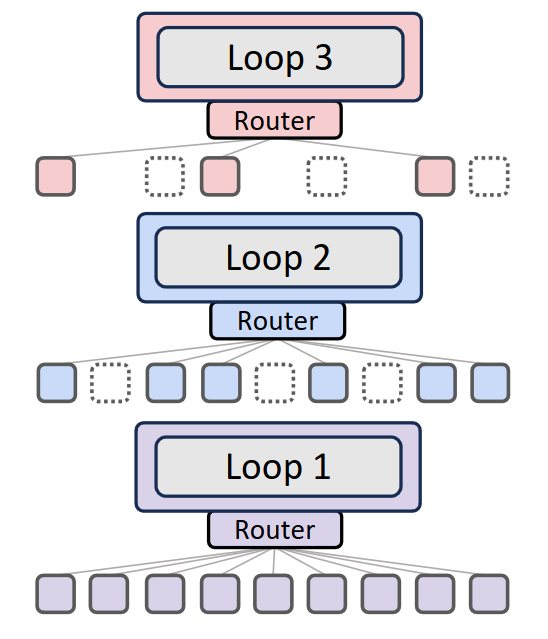
\includegraphics[scale=0.4]{images/expert_choice_routing.png}
  \caption{Routage par choix d'expert \cite{bae2025mixtureofrecursionslearningdynamicrecursive}}
  \label{fig:expert-choice-routing}
\end{figure}

Chaque "étape de récursion" agit comme un expert qui choisit les tokens
qu'il veut traiter. Ce qui permet un contrôle très précis du budget calcul
à chaque étape. On sait exactement combien de tokens sont actifs.

\subsection{Token choice routing}
Le token lui-même, via sa représentation initiale, "choisit" en quelque sorte
combien de calcul il va recevoir. Dès le début, un routeur regarde
la représentation de chaque token et en fonction de cela il assigne
une "profondeur de récursion" (nombre de tour).
 
 \begin{figure}[h]
  \centering
  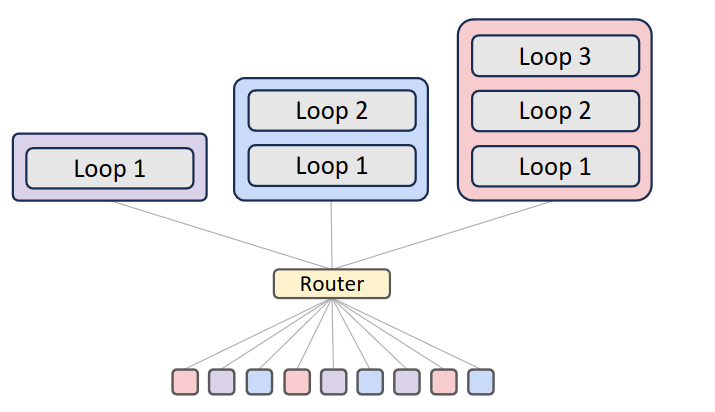
\includegraphics[scale=0.5]{images/token_choice_routing.png}
  \caption{Routage par choix du token \cite{bae2025mixtureofrecursionslearningdynamicrecursive}}
  \label{fig:token-choice-routing}
\end{figure}
 
 Prenons par exemple la phrase suivante :
 \texttt{"Le chat philosophique mange la nourriture délicate."}, pour chaque
 mot, en fonction de leur représentation, le routeur va décider immédiatement
 du nombre de tours qu'il fera.
 
 \begin{itemize}
  \item \texttt{"Le"}, \texttt{"la"} ---> $1$ recursion
  (sort immédiatement après le premier passage, c'est un mot de structure);
  \item \texttt{"chat"}, \texttt{"mange"}, \texttt{"nourriture}" ---> $2$ tours
  (mots normaux);
  \item \texttt{"philosophique"}, \texttt{"délicate"} ---> $3$ tours
  (mots complexes qui nécessitent une "réflexion" profonde).
 \end{itemize}

 À la fin du permier passage, le routeur sélectionne \texttt{"philosophique"},
 \texttt{"délicate"}, \texttt{"chat"}, \texttt{"mange"}. \texttt{"Le"}
 et \texttt{"la"} sortent. Ensuite, à la fin du 2ème passage, le routeur
 sélectionne \texttt{"philosophique"} et \texttt{"délicate"}.
 Les autres sortent. Au 3ème passage, seuls les deux mots complexes restants
 terminent leur traitement.

 Chaque token parcourt le nombre de boucles qui lui a été assigné,
 puis s'arrête. Il n'y a pas de décision à prendre après le départ.
 En effet, c'est le token lui-même, via sa représentation initiale,
 qui "choisit" en quelque sorte combien de calcul il va recevoir.

Les mots simples ont été calculés rapidement, libérant les ressources
pour que le modèle réfléchisse longuement aux mots complexes.
Tout cela en réutilisant le même petit bloc de couches.

% \begin{tcolorbox}[breakable, size=fbox, boxrule=1pt, pad at break*=1mm,colback=cellbackground, colframe=cellborder]
%   % \prompt{In}{incolor}{2}{\boxspacing}
%   \begin{Verbatim}[commandchars=\\\{\}]
% \PY{k+kn}{import}\PY{+w}{ }\PY{n+nn}{os}

% \PY{n+nb}{print}\PY{p}{(}\PY{n}{os}\PY{o}{.}\PY{n}{cpu\PYZus{}count}\PY{p}{(}\PY{p}{)}\PY{p}{)}
%   \end{Verbatim}
% \end{tcolorbox}


%  \cite{bae2025mixtureofrecursionslearningdynamicrecursive}




\subsection{Headings: second level}

\begin{equation}
\xi _{ij}(t)=P(x_{t}=i,x_{t+1}=j|y,v,w;\theta)= {\frac {\alpha _{i}(t)a^{w_t}_{ij}\beta _{j}(t+1)b^{v_{t+1}}_{j}(y_{t+1})}{\sum _{i=1}^{N} \sum _{j=1}^{N} \alpha _{i}(t)a^{w_t}_{ij}\beta _{j}(t+1)b^{v_{t+1}}_{j}(y_{t+1})}}
\end{equation}

\subsubsection{Headings: third level}


\paragraph{Paragraph}


\section{Examples of citations, figures, tables, references}
\label{sec:others}

The documentation for \verb+natbib+ may be found at
\begin{center}
  \url{http://mirrors.ctan.org/macros/latex/contrib/natbib/natnotes.pdf}
\end{center}
Of note is the command \verb+\citet+, which produces citations
appropriate for use in inline text.  For example,
\begin{verbatim}
   \citet{hasselmo} investigated\dots
\end{verbatim}
produces
\begin{quote}
  Hasselmo, et al.\ (1995) investigated\dots
\end{quote}

\begin{center}
  \url{https://www.ctan.org/pkg/booktabs}
\end{center}


\subsection{Figures}

See Figure \ref{fig:fig1}. Here is how you add footnotes. \footnote{Sample of the first footnote.}


\begin{figure}
  \centering
  \fbox{\rule[-.5cm]{4cm}{4cm} \rule[-.5cm]{4cm}{0cm}}
  \caption{Sample figure caption.}
  \label{fig:fig1}
\end{figure}

\begin{figure} % picture
    \centering
    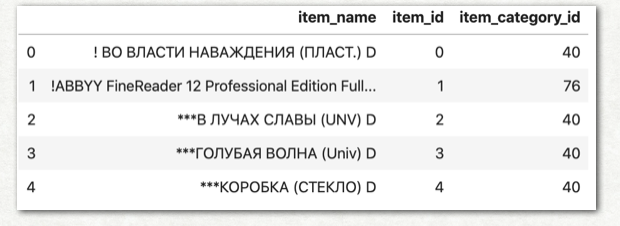
\includegraphics{test.png}
\end{figure}

\subsection{Tables}
See awesome Table~\ref{tab:table}.

\begin{table}
 \caption{Sample table title}
  \centering
  \begin{tabular}{lll}
    \toprule
    \multicolumn{2}{c}{Part}                   \\
    \cmidrule(r){1-2}
    Name     & Description     & Size ($\mu$m) \\
    \midrule
    Dendrite & Input terminal  & $\sim$100     \\
    Axon     & Output terminal & $\sim$10      \\
    Soma     & Cell body       & up to $10^6$  \\
    \bottomrule
  \end{tabular}
  \label{tab:table}
\end{table}

\subsection{Lists}
\begin{itemize}
\item Lorem ipsum dolor sit amet
\item consectetur adipiscing elit.
\item Aliquam dignissim blandit est, in dictum tortor gravida eget. In ac rutrum magna.
\end{itemize}


\bibliographystyle{unsrt}
\bibliography{references}  %%% Remove comment to use the external .bib file (using bibtex).
%%% and comment out the ``thebibliography'' section.


%%% Comment out this section when you \bibliography{references} is enabled.
% \begin{thebibliography}{1}

% \bibitem{kour2014real}
% George Kour and Raid Saabne.
% \newblock Real-time segmentation of on-line handwritten arabic script.
% \newblock In {\em Frontiers in Handwriting Recognition (ICFHR), 2014 14th
%   International Conference on}, pages 417--422. IEEE, 2014.

% \bibitem{kour2014fast}
% George Kour and Raid Saabne.
% \newblock Fast classification of handwritten on-line arabic characters.
% \newblock In {\em Soft Computing and Pattern Recognition (SoCPaR), 2014 6th
%   International Conference of}, pages 312--318. IEEE, 2014.

% \bibitem{hadash2018estimate}
% Guy Hadash, Einat Kermany, Boaz Carmeli, Ofer Lavi, George Kour, and Alon
%   Jacovi.
% \newblock Estimate and replace: A novel approach to integrating deep neural
%   networks with existing applications.
% \newblock {\em arXiv preprint arXiv:1804.09028}, 2018.

% \end{thebibliography}


\end{document}
